\section{Umsetzung des Projektziels}\label{umsetzungProjekt}
Während es sich bei den beiden vorherigen Kapiteln um die Inbetriebnahme des GSM-Netzes selbst gehandelt haben, geht es nun um die konkrete Umsetzung des eigentlichen Projektziels "Man-In-The-Middle". Dabei wird versucht die Gesprächsdaten auf der Strecke zwischen BTS, BSC und der Telefonvermittlungsanlage abzugreifen und zu speichern. Da alle Systeme softwareseitig auf einem PC ausgeführt werden und diese über Sockets miteinander kommunizieren, können die Daten überall abgegriffen werden.\\

Zuerst versucht zwischen BTS und BSC?!?
-> evtl Screenshot von Daten des ABIS-Interface?!
https://osmocom.org/projects/osmo-sip-conector/wiki/Osmo-sip-connector

http://ftp.osmocom.org/docs/latest/osmonitb-usermanual.pdf -> p.6/7 \\

Abgreifen der Daten zwischen BTS und BSC (ABIS-Interface) schwierig -> Daten weiter analysiert und weitere Angriffspunkte ausmachen.
-> Abgreifen der Daten vor der Telefonanlage (Asterisk (OPEN: IAX; Osmo: PBX)) -> dadurch die Daten im VOIP Format (SIP + RTP), welches via PC relativ gut zu handeln ist. \\

Zunächst eigenes analysieren der Daten. Suche nach pratkischem Tool im Internet
-> pcapsipdump\\


Für die Installation und Einrichtung der benötigten Tools wurde ein Bash-Skript erstellt, welches die meisten Schritte automatisch durchführt. Die manuell noch auszuführenden Schritte werden in der Komandozeile ebenfalls ausgegeben (siehe Anhang \ref{configureScript}).


\subsection{Abspeichern der Daten}\label{abspeichern}
Mit Wireshark oder den beiden Komandozeilenanwendungen tshark und tcpdump können Daten von einem Interface in eine pcap-Datei abgespeichert werden. Hierbei können auch bereits beim Aufnehmen Filter gesetzt werden, sodass nur die relevanten Daten gespeichert werden.\\

Pcapsipdump ist ein open-source Tool, welches auf der libpcap basiert. Das Tool hört auf einem Interface den Netzwerkverkehr mit und speichert die SIP/RTP sessions als pcap-Datei ab. Diese Datei kann nun in tcpdump, Wireshark oder ähnlichem geöffnet, eingelesen und weiterverarbeitet werden. Das nette Feature dabei ist, dass das Tool pro Session selbstständig eine Datei anlegt. Das Tool läuft als Hintergrundprozess, sodass es nur einmal manuell gestartet werden muss. Alternativ kann das Tool auch mit dem systemd-Init-Prozess automatisch gestartet werden, sofern man es nachträglich selbst konfiguriert. Da die Tools für das GSM-Netz, wie bereits erwähnt, alle auf dem selben Rechner laufen, reicht es das Loopback-Interface abzuhören.\\

Vor der Installation des Programmes selbst muss Subversion und folgende Abhängigkeit installiert werden.
\begin{lstlisting}
sudo apt-get install -y subversion libpcap-dev
\end{lstlisting}

Das Programm selbst vom SVN-Server herunterladen und installieren.
\begin{lstlisting}
svn checkout https://svn.code.sf.net/p/pcapsipdump/code/trunk pcapsipdump-code
cd pcapsipdump-code
sudo make
sudo make install
\end{lstlisting}

Das Tool kann über das selbst erstellte startingPcapsipdump.sh-Skript oder alternativ auch manuell gestartet werden. Mit angegebenen Parametern lauscht es auf dem Loopback-Interface mit und speichert die Telefongespräche, sobald ein Anruf initiiert wird, in den angegeben Ordner. Des Weiteren werden die Daten immer Paket gepuffert geschrieben, sodass die Datei immer konsistent ist.
\begin{lstlisting}
sudo pcapsipdump -i lo -v 10 -d /home/all/wiresharkCalls/%Y%m%d-%H%M%S-%f-%t-%i.pcap -U
\end{lstlisting}

\subsection{Extrahieren und konvertieren der Daten}\label{extractData}
Zunächst wurden die von pcapsipdump extrahierten Daten mit Wireshark manuell analysiert. Darin sind nun nur noch die SIP- und RTP-Packet enthalten, wie auf fig XXXXX zu sehen. Mit Wireshark erkennt auch den VOIP-Anruf und kombiniert die RTP-Packages korrekt. Allerdings konnte der Stream nicht direkt im Programm abgespielt werden. Der Grund hierfür ist vermutlich, dass Wireshark gsm nicht dekodieren kann.
Jedoch gibt es einen Weg, wie die beiden Streams als .raw-Daten exportiert werden können. Hierfür ein beliebiges RTP-Packet auswählen, über "Telefonie->RTP->Stream Analyse" den Stream analysieren. Nun kann der Hinweg und Rückweg als seperate Datei gespeichert werden. Man muss jedoch als Datei-Typ .raw auswählen.

Die .raw-Dateien können nun via folgendem Komandozeilenaufruf abgespielt werden
\begin{lstlisting}
padsp play -t gsm -r 8000 -c 1 example.gsm
\end{lstlisting}

Mit dem universellen und sehr mächtigen Audiokonverter SoX können die Dateien in .wav convertiert werden, sodass diese auch mit jedem herkömmlichen Media Player abgespielt werden können.
\begin{lstlisting}
sox -t gsm -r 8000 -c 1 example.raw exampleConverted.wav
\end{lstlisting}

Mit dem Bash-Skript pcap2wav von https://gist.github.com/avimar/d2e9d05e082ce273962d742eb9acac16 können genau diese Schritte automatisiert ausgeführt werden.


\subsection{Automatisierung}\label{automatisierung}

Das Abspeichern der Daten funktioniert bereits voll automatisiert und jeweils auch in eine extra Datei pro Session. Allerdings sollte das Konvertierungs-Skript noch automatisch getriggert bzw. ausgeführt werden. Hierfür kann das Linux-Tool \textit{Incron} genutzt werden. Das Tool setzt auf das Kernel-Subsystem Inotify, um auf Dateisystem-Ereignisse zu reagieren. Dadurch kann ein Ordner überwacht werden und zum Beispiel beim erstellen einer neuen Datei etwas getriggert werden, wie eben die Ausführung des Konvertierungs-Skriptes. Incron ähnelt dabei in der Handhabung an das Standardwerkzeug \textit{Cron}, welches Cron Jobs auf Basis von Zeitpunkten startet.


\begin{lstlisting}
sudo apt-get install -y incron
\end{lstlisting}

Damit das Programm gestartet und konfiguriert werden kann, muss in die Datei \textit{/etc/incron.allow} der Username eingetragen werden. Danach kann der Service gestartet werden.

\begin{lstlisting}
systemctl start incron.service
\end{lstlisting}

Pinzipiell gleich wie bei \textit{Cron} werden über \textit{incrontab -e} die Jobs angelegt und verwaltet.
\begin{lstlisting}
/home/all/wiresharkCalls IN_CLOSE_WRITE /home/all/startPcap2wavgsmConversion.sh $@ $#
\end{lstlisting}


\begin{figure}[h] %t=top b=bottom h=here p =eigene page
\centering
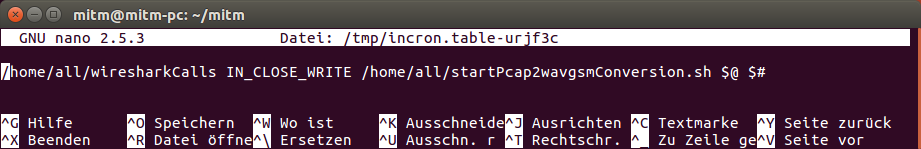
\includegraphics[width=15cm]{includes/incrontab}
\caption{Zeile des incrontab}
\label{fig:incrontab}
\end{figure}


Der Eintrag besteht aus dem Pfad, des zu beobachtenden Verzeichnisses, dem auftretendem Ereignis und zuletzt den auszuführenden Befehl beziehungsweise Skript. Über den Parameter \textit{\$@}  wird das beobachtete Verzeichnis und mit \textit{\$\#} den Namen der Datei, welches das Ereignis getriggert hat, übergeben. Damit das Konvertierungs-Skript von \ref{extractData} erst ausgeführt wird, wenn alle Daten geschrieben worden sind, wurde das Ereignis \textit{IN\_CLOSE\_WRITE} genutzt, wie in Abbildung \ref{fig:incrontab} zu sehen. Das Skript wird nun getriggert, sobald die Datei vom Schreiben geschlossen wurde.\\

Über den Status kann überprüft werden ob ein Ereignis ausgelöst und der Befehl getriggert wurde.

\begin{lstlisting}
systemctl status incron.service
\end{lstlisting}


Nun werden also die Daten direkt von der Schnittstelle abgegriffen, gefiltert und gespeichert. Danach automatisch in .wav konvertiert, sodass die Gespräche lokal auf dem PC angehört werden können. Damit wäre das Projektziel bereits erreicht beziehungsweise mit der Konvertierung auch praktisch erweitert. Um nicht an den lokalen PC gebunden zu sein, wäre es nun auch möglich die Dateien über einen Webserver global zur Verfügung zu stellen.

\subsection{Feature - Abhören der Aufnahme}
Es soll das letzte oder die letzten Gespräche via einem Telefonanruf wiedergegeben werden können. Dies wurde mit einer/mehreren speziell konfigurierten Nummern ermöglicht.

-> aktuelle extensions.conf ziehen


\subsection{Aufgetretene Probleme}

Aufnehmen der Daten -> zunächst nur UDP -> in Wireshark Protokoll rtp\_udp aktivieren -> Streams reichen nicht aus? (um alles automatisieren?!?) -> Installation von Sip-Connector\\

Konfigurationsprobleme -> Config Files bei einem System funktionieren auf dem eig. gleichen System auf einmal nicht mehr\\

Bei Osmocom treten allgemein manchmal Verzögerungen beim Auflagen sowie je nach Telefon auch Störgeräusche auf.\\



Mit dem Tool in \ref{extractData}, welches für das Abspeichern der Daten zuständig ist, gab es Probleme. Denn es wurde kein Datei-Ereignis beziehungsweise erst nach sehr langer Verzögerung erkannt. Nach Lesen und Debuggen des Source-Codes, stellte sich heraus, dass das Tool die erstellte Datei lange nicht schließt, obwohl bereits seit längerem die Session beendet ist. Der Übeltäter war ein Timer in der calltable-Klasse, welcher auf 5 Minute gestellt war. Nach Verändern des Source-Codes und Anpassen des Timers auf 5 Sekunden wurde auch die erstellte pcap-Datei kurz nach Ende der Session geschlossen und das Incron-Ereignis getriggert.

\begin{lstlisting}[xleftmargin=.04\textwidth, firstnumber=211]
  ...
 if (table[idx].is_used && (
 	(currtime - table[idx].last_packet_time > 5) ||
    (currtime - table[idx].first_packet_time > opt_absolute_timeout))){
  ...
\end{lstlisting}
